\chapter{A Middleware for Secure Aggregation of Data in Solid}
\label{cha:solution-overview}
This chapter introduces the architecture of \middleware{} (Middleware for Aggregation Security and protection in Solid): a middleware for performing secure and protected data aggregation on top of the Solid protocol. This section starts with a discussion of what the general architecture for such data aggregation looks like, and indicating which concrete problems occur in such an architecture. Based on the use cases described in section \ref{sec:usecases}, a number of requirements for the middleware are formed. Thereafter, the architecture of the middleware is discussed followed by an in-detail explanation of its components. The concrete implementation of this middleware is discussed in the next chapter.

\section{A Generic Data Aggregation Architecture in Solid}
A middleware for aggregation in Solid will consist of a number of components, each with their own responsibility. Figure \ref{fig:reference-architecture} illustrates a reference architecture of a data aggregation system in Solid. 

\begin{figure}[h]
    \centering
    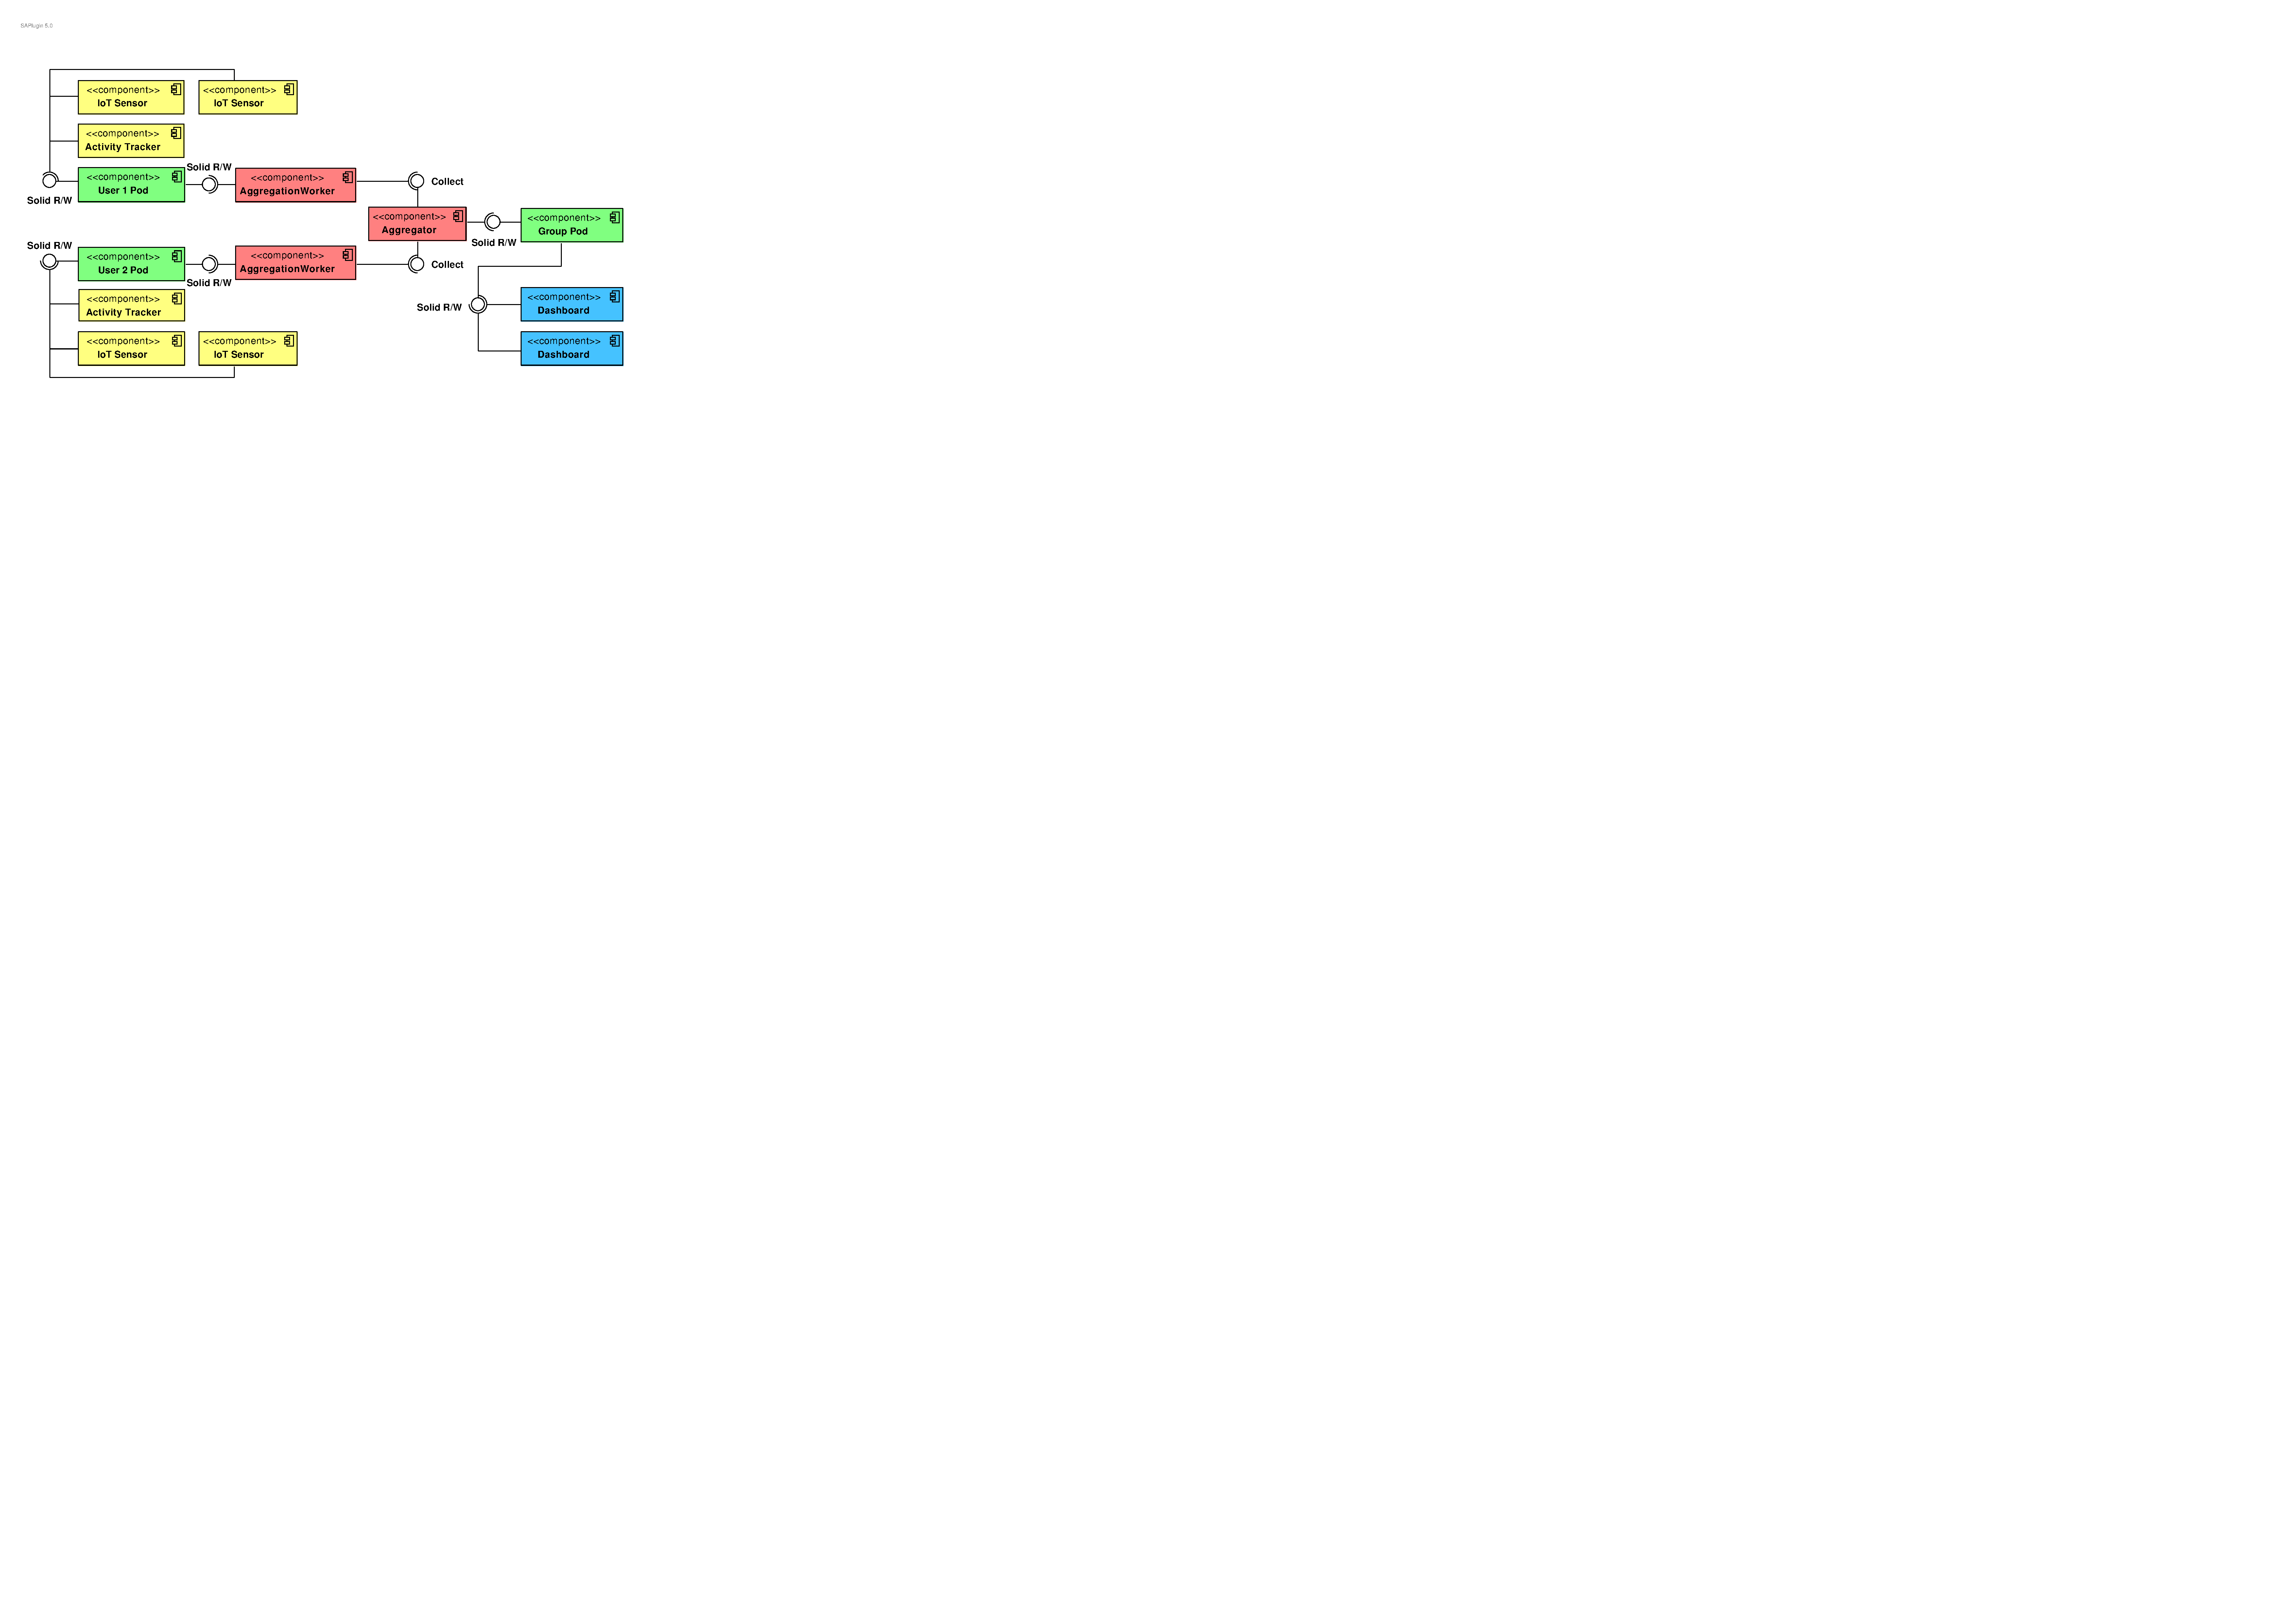
\includegraphics[width=1.0\textwidth]{images/architecture/Reference-Architecture-Aggregator.pdf}
    \caption{Reference architecture for data aggregation in Solid}
    \label{fig:reference-architecture}
\end{figure}

\noindent This reference architecture highlights a number of challenges that make aggregation insecure, unscalable or privacy-invasive. Concretely, the following issues are remarked.

\begin{enumerate}
    \item IoT Sensors and Activity Trackers are embedded devices that very regularly write data to a Solid Pod. As these are resource-constrained devices, those write operations must be very efficient. As section \ref{sec:dpop} explains, the currently used mechanism uses public key cryptography, which is very computationally expensive.
    \item The aggregator component (illustrated in red on the figure) reads complete resources directly from the user's Pod. Privacy-wise, this is unsafe and unnecessary, as not all data present in the resource may be necessary for performing the aggregation. Some method of restricting the data exposed to the aggregator must be devised.
    \item The aggregator component can consist of multiple worker nodes in different networks. Similarly, services can require data from a Solid Pod but also depend on other services that also need access to this data. This is currently not supported in Solid, and existing flows (such as OAuth On-Behalf-Of) impose bottlenecks on the token endpoint. 
    \item Group Pods holding data of users from different Pod providers are not supported as of yet. This comes with challenges in the authentication domain.
\end{enumerate}

\noindent All of these problems are situated (at least partially) in the domain of the Solid server, which provides the user's pods. A number of improvements here could help alleviate the problems listed above. The problems listed above can be divided in two categories: resource management and authentication management. To solve these problems, a solution will need to consist of two parts: one focused on rendering exposed resources more private, the other focused on improving the authentication mechanism. In order to develop a solution that is sufficient, first an attacker model and a number of requirements are presented. Afterwards, an overview of the conceptual solution is presented. The components of this solution are then discussed in more detail.

\newpage
\subsection{Adversary model}
\label{sec:attacker-model}
The attacker model considered in the design and development of \middleware{} handles the case of untrusted aggregators and applications. Untrusted in this case means that the user wishes to use the aggregator or application, but wants to minimize the amount of data exposed to it. Thus, the adversary is a Solid application to which the user grants access. Concretely, this means that the application can access any data to which the \gls{ACL}s give it access, and in the modes determined herein. However, there is no fine-grained privacy control, i.e., on the level of a single resource. Consequently, the attacker here is an honest-but-curious attacker, which does not deviate from the Solid protocol and does not attempt to break the access control mechanisms.

It is important to note the goal of \middleware{} in terms of disclosure prevention here. As explained in section \ref{sec:statistical-privacy}, many \gls{PETs} try to prevent identity disclosure (in datasets containing data from many different users). However, since every Solid pod is linked to a WebID (containing data of a single user), the main goal of this middleware is to prevent attribute disclosure. Accordingly, the attackers considered in the two adversary models try to gain knowledge of \textit{data attributes}. Handling identity disclosure is also an important aspect of a privacy-aware software system (and especially for data aggregators), but in the case of Solid, this must be handled by data aggregators and other clients collecting data over multiple pods themselves.

\subsection{Requirements}
\label{sec:requirements}

\subsubsection{Functional requirements}
\noindent \textbf{Flexibility for the supported data scheme} Solid builds further upon the principles of Linked Data, and Solid servers can store nearly any type of data. As \middleware{} aims to be a general solution, it should work with any type of structured data, i.e., it must provide a way to anonymize \textit{any} type of textually represented structured data. Thus, flexibility for the supported data scheme is an essential part of \middleware{}. Concretely, \middleware{} should not hard-code any supported data schemes nor which PET should be applied to them: these should be able to be plugged in flexibly and selected automatically, to ensure that any data scheme can be supported. This provides a technical challenge, as a sufficient level of abstraction must be developed to be able to support any data scheme, while ensuring that the leakage requirements are not violated. \\

\noindent \textbf{Automatically select \gls{PETs}} Different applications may be trusted differently, just as different data schemes may contain more or less sensitive data elements. An important aspect to solve is thus being able to distinguish different \textit{privacy levels}: required levels of anonymization. \middleware{} must therefore not only be able to adapt to different data schemes, but must also support different privacy levels for every data scheme. The selected PET is highly dependent on the data scheme and required level of privacy, therefore \middleware{} must automatically select \gls{PETs} based on the input data scheme and requested privacy level. \\

\noindent \textbf{Extensibility} Finally, the Solid project is still very much a work in progress. This implies that the specification will likely be modified many times in the future, and additional features will be added. If \middleware{} wants to successfully keep interacting with Solid servers, the architecture should be ready to easily be extended in order to support newly released features and modifications. \\

\noindent \textbf{Decentralized access token delegation} As aggregators may consists of multiple worker nodes, or they may be dependent of other services, the middleware solution must also enable a mechanism for decentralized access token delegation. In other words, an application must be able to delegate its access token without having to request a new token at the token endpoint. The user should explicitly give access for this.

\subsubsection{Non-functional requirements}
\textbf{Intuitive to use} Solid aims to become the de-facto standard for web applications in the future. Consequently, it must be intuitive for non-technical users to use this technology. There can be no technical jargon, and it must be incredibly easy to set-up. Since \middleware{} aims to follow this philosophy, the proposed solution must be intuitive to use for non-technical users. 

Concretely, this means that it should be opaque to the users which concrete PET is applied for which use case. On that account, a number of \textit{privacy levels} should be created and presented to the user in a simple manner: a higher privacy level means more data protection but less utility. The user will then be able to select between a number of privacy levels, without needing to understand the technical details behind the scenes. Examples of concrete transformations can be given, to make the effects of selecting a certain level more comprehensible. \\

\noindent \textbf{Testability} Since \middleware{} operates so dynamically, there is a lot of opportunity for bugs to sneak in that will go unnoticed. Some bugs may only appear under the presence of a specific combination of transformations in the configuration files. Therefore, testability is an important aspect. Increased testability gives stronger guarantees of the correct behavior of \middleware{}, which is essential in the context of a privacy-enhancing technology. \\

\noindent \textbf{Minimal overhead} Since \middleware{} operates as a middleware, it will be called on every resource request. The overhead associated with this should be minimized, such that the used Solid server does not become unusable due to running the middleware.

\newpage
\section{Conceptual Middleware Architecture}
To solve the problems and fulfill the requirements stipulated above, \middleware{} consists of two main components. The first component is called \textit{privacy filters} and focuses on improving data privacy for data exposed to aggregators (or other applications). The second component is an implementation of macaroons in Solid, i.e. a new access token mechanism. This mechanism supports decentralized delegation, group vaults, and is computationally efficient (to support data writes by IoT sensors, ...).

Privacy filters are a mechanism to dynamically modify requested resources to strip away or modify sensitive data attributed. When a resource is requested for aggregation, it often contains a lot of unnecessary and private information. Privacy filters are implemented as a middleware in the Solid server, and dynamically strip away certain attributes of the resource. To realize this, a number of configuration files are loaded on to the server, or the user's pod. These configuration files describe what \textit{privacy tactics} ought to be applied to a certain data scheme. The configuration files contain a number of privacy tactics for every \textit{privacy level}. Privacy levels are a granular way to select how much to trust a certain application / aggregator. The higher the privacy level, the more privacy (and in turn, less data utility). Privacy filters are discussed in detail in the next chapter. 

To alleviate the authentication and authorization problems that come with data aggregation in Solid, this thesis investigates the use of macaroons in Solid. Some background information on macaroons has been given in section \ref{sec:macaroons}. Macaroons support decentralized delegation out-of-the-box, and also support \textit{caveats} (requirements which must be fulfilled for a token to be valid), as well as third-party attestations. These properties can improve aggregation security, for example by embedding the required privacy level inside the access token. Furthermore, in this manner the access tokens can be restricted to a single resource on the token side. Lastly, macaroons use \acrlong{HMAC} instead of public-key cryptography. This creates performance improvements for allowing IoT devices or activity trackers to write to Solid pods. The integration of macaroons in Solid is discussed in detail in chapter \ref{cha:macaroons-solid}.

It is clear that the combination of these two components can enable better and more secure data aggregation in Solid. Figure \ref{fig:aggregation-flow} illustrates more concretely the flow of data aggregation using these two new mechanisms.

\begin{sidewaysfigure}
    \centering
    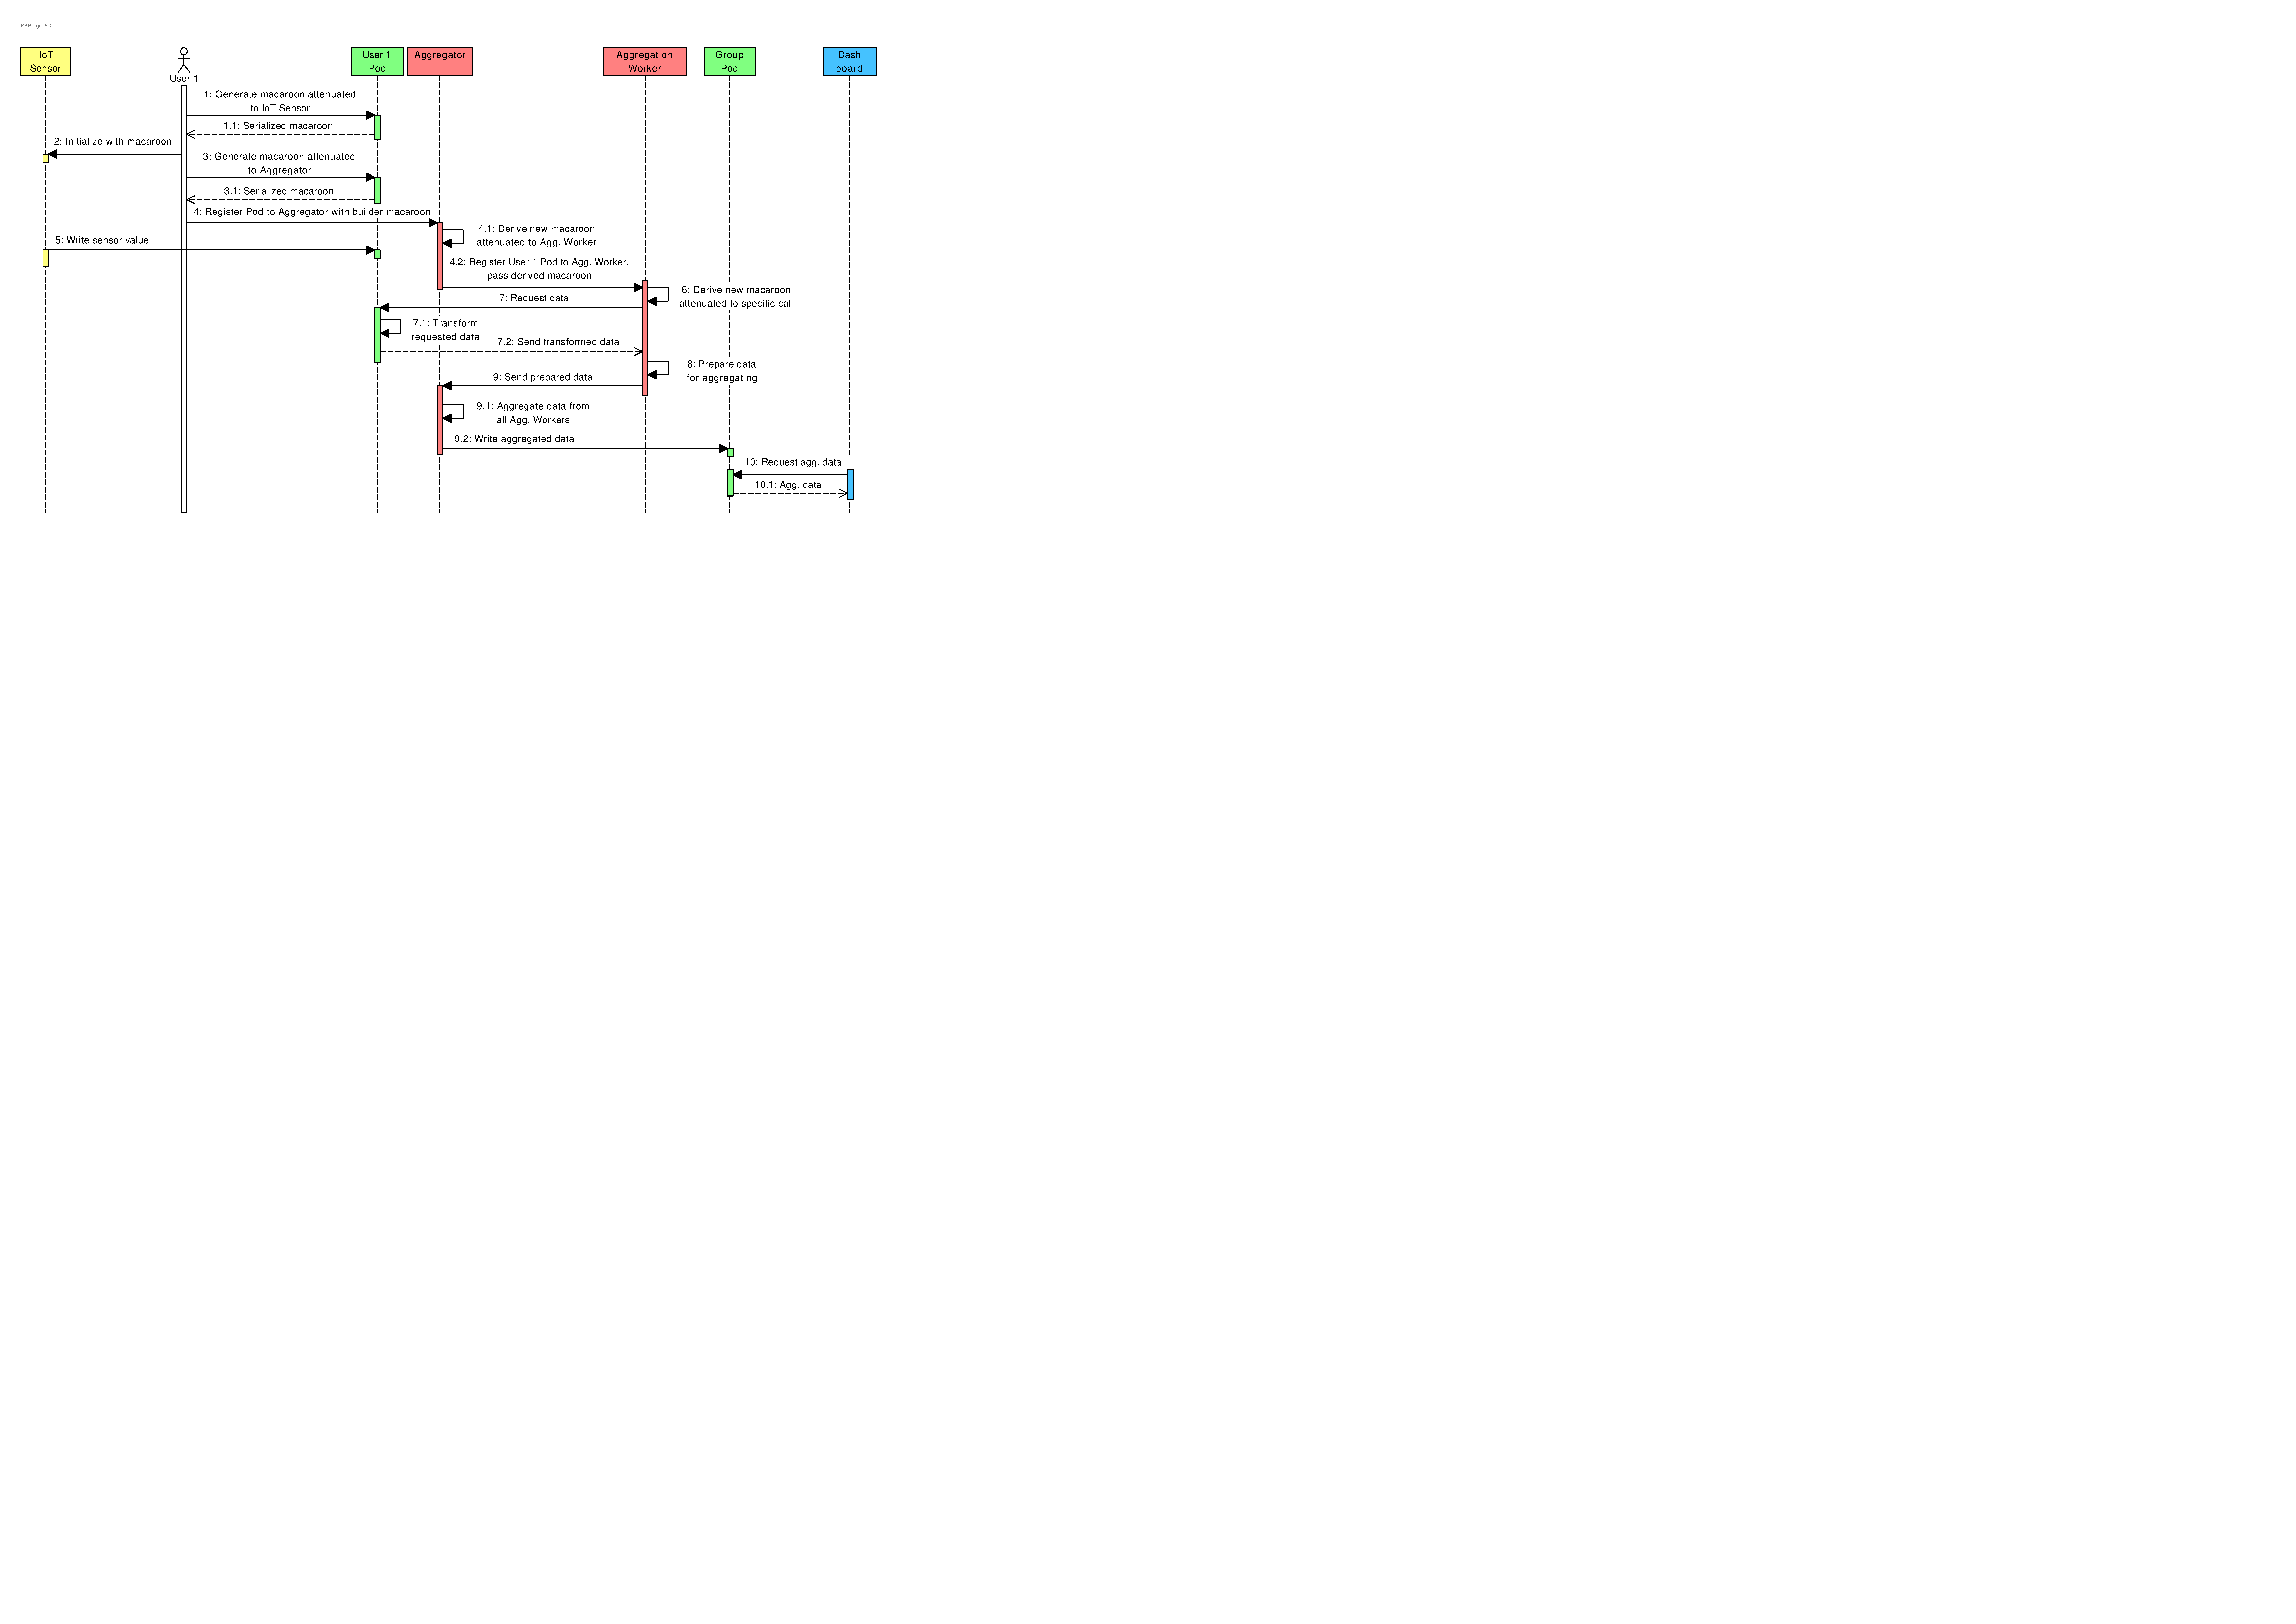
\includegraphics[width=1.0\textwidth]{images/architecture/InteractionDiagram-Aggregation-flow.pdf}
    \caption{Aggregation flow}
    \label{fig:aggregation-flow}
\end{sidewaysfigure}

%\section{Privacy Filters}
%\label{sec:privacy-filters}
%The goal of this section is to find a solution to the information leakage problems that come with data aggregation. This problem arises due to the fact no distinction is made between the trust level given to client applications in Solid. These applications either get the full resource or nothing, but since mostly structured data is handled by Solid, it should be possible to restrict which parts of a resource are exposed.

%As illustrated by figure \ref{fig:privacy-utility-tradeoff}, improved privacy always comes with a trade-off regarding data utility. Evidently, data with less or less precise attribute values will be more private, but this same property also renders the data less useful. Making this trade-off is very context-dependent (how much is the application trusted, what kind of data is requested etc.). As such, rendering data more private must happen dynamically, at the time of a request, such that details of the request can be taken into account when determining what kind of transformations ought to happen to the data.

%\begin{figure}[h]
%    \centering
%    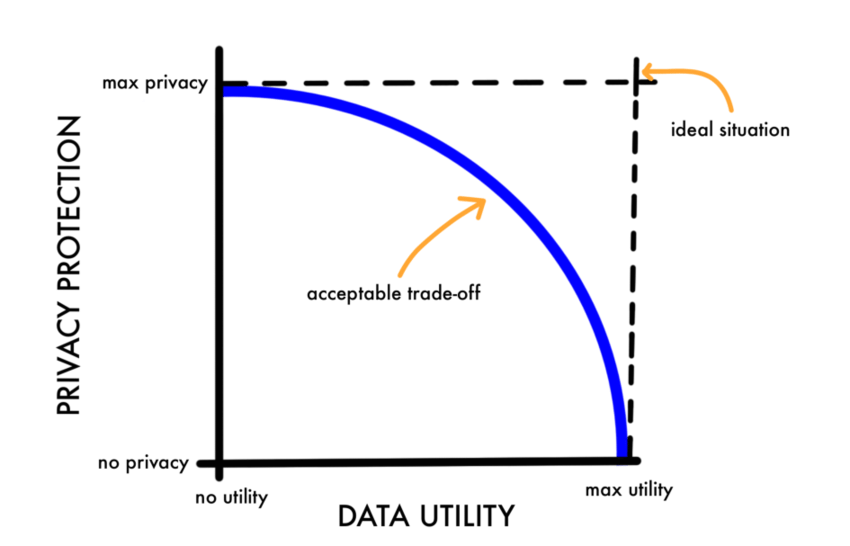
\includegraphics[width=0.8\textwidth]{images/Data-Privacy-Protection-versus-Data-Utility.png}
%    \caption{Illustration of the privacy-utility trade-off, from \citet{datasharing-implications}}
%    \label{fig:privacy-utility-tradeoff}
%\end{figure}

%\noindent This section introduces the concept of \textit{privacy filters}, which dynamically strip away attributes of exposed data in accordance with some predefined rules. A prototype middleware is developed which implements, along with macaroons, privacy filters. The concrete implementation is discussed in chapter \ref{cha:middleware}.

%Conceptually, this mechanism works as follows. Users load a number of privacy filter configuration files, which specify what transformations must happen to what datatype. Users can then specify how much privacy they want (in general, or for specific datatypes, see next section). When a request is received, \middleware{} checks the data type of the requested resource and the requested level of privacy. Subsequently, a number of transformations are applied to the data (as specified by the privacy filter configuration file), after which the transformed data is returned to the application. An example of what such a rewrite can look like is provided in figure \ref{fig:example-treatment-privacy-filter}.

%\noindent Privacy filters are represented by a configuration file for every filter. This configuration file describes the privacy tactics that must be applied to resources of a certain datatype. An example of such a configuration file is shown in the appendix, in listing \ref{listing:privacy-filter-kbc}.

%\subsection{Privacy levels}
%\label{sec:privacylevels}
%\noindent In order to provide an intuitive mechanism for selecting which data is transformed, the concept of privacy levels is introduced. Privacy levels form an abstraction above the concrete data transformations and \gls{PETs} that are applied to the data before it is passed on to the application. This ensures that non-technical users can use a privacy-enhancing middleware, without needing to understand the technical details of the technologies and tactics that are employed. 

% \middleware{} is configured with a default privacy level, but also supports specific privacy levels for certain data schemes. For example, a user could configure \middleware{} to use privacy level 2 by default, but privacy level 4 on bank transactions, since he does not want to expose this data. This makes the middleware more context-sensitive and allows for strong configurability. The privacy-utility trade-off can then also be taken into account for specific applications that need data with very high utility to deliver usable results. For every data scheme, an explanation should also be included which specifies concretely what will happen to the data under a certain privacy level.

% Another important aspect is that the developers of privacy filters for specific data schemes must be aware of what privacy levels map to what leakage or tactics. This is best determined by privacy experts as it is a very complex topic. However, appendix \ref{appendix:privacy-levels} shows an example of such a mapping that was used to guide the development of configuration files for the prototype of \middleware{}.



% \subsubsection{Supported transformations}
% Table \ref{table:supported-transformations} gives an overview of which transformations are currently supported in \middleware{}. The choice for supported transformations is mostly based on the discussion from section \ref{sec:transformation-approaches}. This section discussed a taxonomy of architectural tactics involving data transformations. Some tactics could not be mapped to an equivalent tactic in our middleware because the middleware works on a per-request basis. An example of this is the \textit{Select / Filter} tactic, which keeps a copy of the original data. The \textit{Aggregate} tactic was not applicable as \middleware{} does not support grouping data elements, as data is treated on a per-attribute basis. Similar arguments hold for other tactics that are not supported. The \textit{Perturbation} tactic is based on the \textit{Blur} tactic from table \ref{table:de-id-taxonomy}, but renamed to convey its applicability to numeric values. Similarly, \textit{Encrypt} is supported along with the similar \textit{Hash} tactic.

% \begin{table}[H]
\begin{center}
\begin{tabulary}{\textwidth}{p{0.20\textwidth}p{0.8\textwidth}}
\textbf{Transformation name} & \textbf{Description}                                                                                                                                                          \\ \hline
Remove               & The targeted and deliberate omission of PII from the data record or data set.                                                                                                 \\
Pseudonym            & The systematic replacement of direct identifiers with surrogates, whereby the mapping between surrogate and identity is kept separately.                                      \\
Perturbation         & The insertion of randomized noise into the values of the data to hide exact values                                                                                 \\
Random               & Tactics that involve the modification of PII attribute values/records by injecting artificial random elements.                                                                \\
Encrypt              & Using cryptographic means to encode the PII attribute values / records / datasets.                                                                                            \\
Hash                 & Using cryptographic hash functions to obfuscate the PII attribute values / records / datasets in a deterministic fashion.                                                                                            \\
\end{tabulary}
\caption{Overview of data transformations supported in \middleware{}}
\label{table:supported-transformations}
\end{center}
\end{table}
